\chapter{Teil 2: Klassifikation}
\section{Einleitung}
Um eine Klassifizierung durchführen zu können, sind mehrere Komponenten notwendig, welche miteinander arbeiten. 
Dieser Ablauf wird in der \cref{fig:ablauf_klassifizierung} gezeigt.
\begin{figure}[H]	
	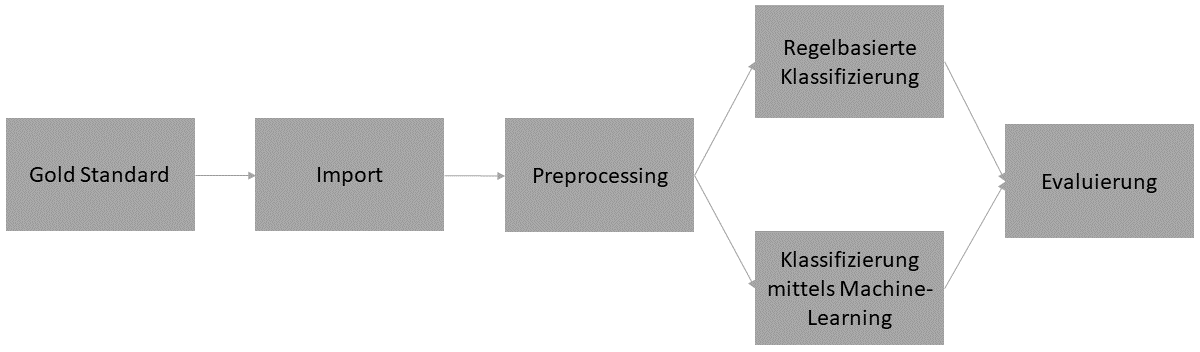
\includegraphics[width=1\columnwidth,keepaspectratio]{img/Ablauf_Klassifizierung.png}
	\caption{Pipeline}
	\label{fig:ablauf_klassifizierung}
\end{figure}
Als Grundlage dienen die Daten des Gold Standards.
Diese werden mittels einer Import-Komponente geladen.
Bevor die Daten mit den entsprechenden Methoden klassifiziert werden, werden sie bei Bedarf noch vorverarbeitet.
Dann findet die eigentliche Klassifizierung statt.
Um eine möglichst präzise und erfolgreiche Variante des Klassifizierens zu finden, werden in diesem Teil der Arbeit mehrere Experimente durchgeführt.
Zum Schluss folgt eine Komponente, welche für das Auswerten der Klassifizierung und Ausgeben der Ergebnisse verantwortlich ist.
\section{Preprocessing}
Das Preprocessing wurde entwickelt, um den Inhalt des Dokuments auf eine standardisierte Form zu bringen.
Die folgenden Methoden können sowohl auf den Text eines Dokuments sowie auch auf den Titel angewendet werden.
Sie können mittels Konfiguration sowohl für den Text als auch Titel eines Dokuments ein- oder ausgeschaltet werden.
\subsection{Basis Preprocessing}
\subsubsection{Gross-/Kleinschreibung}
Alle Buchstaben, welche grossgeschrieben sind, werden durch die entsprechenden Kleinbuchstaben ersetzt.
\subsubsection{Umlaute ersetzen}
Umlaute werden durch ihre verwandten Selbstlaute ersetzt, genauer:
\begin{itemize}
	\item ä $\rightarrow$ a
	\item ö $\rightarrow$ o
	\item ü $\rightarrow$ u
\end{itemize} 
\subsubsection{Sonderzeichen entfernen}
Alle Sonderzeichen, die nicht in der folgenden Auflistung vorkommen, werden durch einen Leerschlag ersetzt:
\begin{itemize}
	\item éàèÉÀÈäöüÄÖÜa-zA-Z
\end{itemize} 
\subsubsection{Einzelne Zeichen entfernen}
Jedes einzelne Zeichen, also solche, die sowohl vorne als auch hinten an einen Leerschlag angrenzen, werden entfernt.
\subsubsection{Multiple Leerschläge entfernen}
Da durch die vorhergehenden Schritte oft multiple Leerschläge anfallen, werden diese auf einen Leerschlag reduziert.
\subsection{Erweiterte Preprocessing}
\subsubsection{Preisdetektor}
Da Menüs häufig in Verbindung mit Preisen vorkommen und in weiteren Preprocessing-Schritten Zahlen und Sonderzeichen entfernt werden, ist es von Vorteil, diese Informationen nicht zu verlieren.
Daher erkennt diese Methode verschiedene Varianten von Preisen mittels Regulären Ausdrücken (Regex, Regular Expression) und ersetzt diese mit einem Schlüsselwort.
% Varianten genauer ausführen
Die folgenden Varianten von Preisen wird erkannt:
\begin{itemize}
	\item Preisangabe + chf/fr/sfr
	\item Preisangabe
	\item chf/fr/sfr + Preisangabe
\end{itemize} 
Zudem wird unterschieden, wie viele Stellen der Preis hat.
Die nun aufgeführte Liste zeigt die verschiedenen Schlüsselwörter:
\begin{itemize}
	\item Einstellig $\rightarrow$ onedigitprice
	\item Zweistellig $\rightarrow$ twodigitprice
	\item Dreistellig $\rightarrow$ threedigitprice
\end{itemize} 
Um Zeitangaben nicht als Preise zu erkennen, werden bei Preisangaben ohne Währungsangabe nur Beträge mit Rappenbeträgen, welche 60 oder höher sind, erkannt.
\subsubsection{Stammformreduktion}
Dieses Verfahren führt verschiedene morphologische Varianten eines Wortes auf ihren gemeinsamen Stamm zurück.
Dafür wird der Stemmer \glqq Cistem\footnote{\url{https://github.com/LeonieWeissweiler/CISTEM} abgerufen am: 18.03.2019}\grqq{} verwendet, da für die deutsche Sprache nur wenig Alternativen vorhanden sind. 
\subsubsection{Getränkedetektor}
% Referenz Cistem
Eine Liste mit Einträgen diverser Getränke bildet die Grundlage dieser Methode.
Wenn im Text ein Getränk dieser Liste vorhanden ist, wird es durch das Schlüsselwort \glqq beverageentity\grqq{} ersetzt.
Damit soll erreicht werden, dass ein einheitliches Merkmal geschaffen wird.
\subsubsection{Stoppwörter entfernen}
Bei Stoppwörter handelt es sich um Wörter, welche keine Relevanz für den Inhalt eines Texts haben, aber oft vorkommen.
Eine Stoppwortliste führt 1720 solcher Wörter in deutsch auf. Sie ist aus mehreren Quellen zusammengesetzt worden.
Wenn eines dieser Wörter im Text vorkommt, wird es entfernt.
\section{Experimente}

\subsection{Regelbasierte Experimente}
\subsubsection{Regelsatz: Menü im Titel}
\paragraph{Beschreibung der Komponente}
\paragraph{Methoden}
\paragraph{Resultate}
\subsubsection{Regelsatz: Preisdetektor}
\paragraph{Beschreibung der Komponente}
\paragraph{Methoden}
\paragraph{Resultate}
\subsubsection{Regelsatz: Kombination aus Menü im Titel und Preisdetektor}
\paragraph{Beschreibung der Komponente}
\paragraph{Methoden}
\paragraph{Resultate}
\subsubsection{Regelsatz: Listing}
\paragraph{Beschreibung der Komponente}
\paragraph{Methoden}
\paragraph{Resultate}
\subsubsection{Regelsatz: Bag of Words}
\paragraph{Beschreibung der Komponente}
\paragraph{Methoden}
\paragraph{Resultate}
\subsubsection{Diskussion der regelbasierten Experimente}
\subsection{Experimente mittels Machine-Learning}
\subsubsection{Dimensionsreduktion der Features}
\paragraph{Beschreibung der Komponente}
\paragraph{Methoden}
\paragraph{Resultate}
\subsubsection{Angabe von Klassenverteilung}
\paragraph{Beschreibung der Komponente}
\paragraph{Methoden}
\paragraph{Resultate}
\subsubsection{Anwendung von N-Gramme}
\paragraph{Beschreibung der Komponente}
\paragraph{Methoden}
\paragraph{Resultate}
\subsubsection{Anwendung von einfachen Preprocssingschritten}
\paragraph{Beschreibung der Komponente}
\paragraph{Methoden}
\paragraph{Resultate}
\subsubsection{Anwendung von fortgeschrittenen Preprocssingschritten}
\paragraph{Beschreibung der Komponente}
\paragraph{Methoden}
\paragraph{Resultate}
\subsubsection{Anzahl extrahierter Features}
\paragraph{Beschreibung der Komponente}
\paragraph{Methoden}
\paragraph{Resultate}
\subsubsection{Hyperparametertuning}
\paragraph{Beschreibung der Komponente}
\paragraph{Methoden}
\paragraph{Resultate}
\subsubsection{Diskussion der regelbasierten Experimente}
\section{Diskussion}
\section{Beantwortung der Forschungsfrage}